% main_report30.tex
% SAMBP TR-30/2026: Cross-Polarised Mho Characteristic for IBR Networks
% Companion to TR-29 (IBR Apparent Impedance Trajectory Analysis)
%
% Compile: pdflatex → bibtex → pdflatex × 2

\documentclass[11pt,a4paper]{article}

%% ── Packages ────────────────────────────────────────────────────────────────
\usepackage[T1]{fontenc}
\usepackage[utf8]{inputenc}
\usepackage[a4paper, margin=25mm]{geometry}
\usepackage{amsmath,amssymb}
\usepackage{booktabs,array,colortbl,tabularx,longtable}
\usepackage{graphicx}
\usepackage{xcolor}
\usepackage{hyperref}
\usepackage{pgfplots}
\pgfplotsset{compat=1.18}
\usepackage{tikz}
\usetikzlibrary{arrows.meta, decorations.pathreplacing, patterns, calc, shapes.geometric}
\usepackage{caption}
\usepackage{subcaption}
\usepackage[expansion=false]{microtype}
\usepackage{parskip}
\usepackage{enumitem}
\usepackage{cite}

%% ── Colours ─────────────────────────────────────────────────────────────────
\definecolor{sambpblue}{RGB}{0,70,140}
\definecolor{sambpgreen}{RGB}{0,120,60}
\definecolor{sambpred}{RGB}{160,30,30}
\definecolor{headerbg}{RGB}{230,238,250}

%% ── Header / Footer ─────────────────────────────────────────────────────────
\usepackage{fancyhdr}
\pagestyle{fancy}
\fancyhf{}
\rhead{\small SAMBP TR-30/2026 --- Confidential Draft}
\lhead{\small Cross-Polarised Mho for IBR Networks}
\cfoot{\small \thepage}

%% ── Title ───────────────────────────────────────────────────────────────────
\title{%
  \textbf{\Large SAMBP Technical Report TR-30/2026}\\[6pt]
  \textbf{\large Cross-Polarised Mho Characteristic for IBR Networks}\\[4pt]
  \normalsize PhD Thesis Supporting Report --- Distance Relay Series II
}
\author{PhD Candidate}
\date{April 2026}

% ─────────────────────────────────────────────────────────────────────────────
\begin{document}
\maketitle\thispagestyle{fancy}

% ── Abstract ─────────────────────────────────────────────────────────────────
\begin{abstract}
TR-29 demonstrated that IBR-fed line faults produce relay voltages below
0.010\,pu for all combinations of current-limit factor $k_\mathrm{ibr}$ and fault
location $\alpha$, invalidating self-polarised Mho operation for the entire IBR
parametric envelope.  This report provides the complementary analysis:
cross-polarisation theory is formalised, the memory-polarised criterion is shown
to be independent of the memory decay magnitude, and the Zone~1 timing margin is
quantified at $5\times$ ($T_\mathrm{mem}/t_{Z1} = 100/20$\,ms).  A full fault-type
matrix is developed showing that Zone~2 and Zone~3 are viable for all non-3PH
faults via permanent healthy-phase cross-polarisation, but remain unavailable for
3-phase faults where only memory polarisation is possible.  Load encroachment is
shown to be inherently safe for leading (capacitive) IBR loads, which always
appear below the $R$-axis, outside the upper-half-plane Mho circle.  The combined
result --- cross-polarised Zone~1 for all faults, and Zone~2/3 for non-3PH via
healthy-phase cross-pol, backed by the 21/21-selective 87L chain --- is the
recommended protection scheme for IBR-fed transmission lines on this network.
\end{abstract}

\tableofcontents\newpage

% =============================================================================
\section{Introduction and Scope}
\label{sec:intro}
% =============================================================================

The SAMBP distance relay series began with TR-18 (Mho zone reach verification
under synchronous-generator feed), then TR-29 identified three failure modes when
the source is replaced by an IBR:
\begin{enumerate}[label=(\roman*)]
  \item \textbf{$I_\mathrm{min}$ blocking} ($k_\mathrm{ibr}<0.10$\,pu) --- relay
        inhibited before polarisation is even attempted;
  \item \textbf{Relay voltage deficiency} ($|V_\mathrm{relay}|\leq 0.010$\,pu) ---
        self-polarised Mho fails for all IBR scenarios;
  \item \textbf{Memory expiry for Zone~2/3} ($T_{Z2/3}>T_\mathrm{mem}$) --- even with
        memory polarisation, Zones 2 and 3 cannot trip 3-phase IBR faults.
\end{enumerate}

This report addresses failure mode (ii) systematically and provides the
cross-polarisation solution, then maps failure mode (iii) onto fault type.
Failure mode (i) is addressed by the 87L chain (TR-23 through TR-27).

\paragraph{Network and relay parameters (unchanged from TR-18/TR-29).}
$Z_\mathrm{src}=j0.10$\,pu, $Z_\mathrm{line}=j0.05$\,pu, $V_\mathrm{pre}=1.00$\,pu.
Zone reaches: $X_{R1}=0.040$, $X_{R2}=0.060$, $X_{R3}=0.090$\,pu.
Trip timers: $t_1=20$\,ms (instant), $t_2=300$\,ms, $t_3=600$\,ms.
Memory hold: $T_\mathrm{mem}=100$\,ms (IEC~60255-121 \cite{IEC_60255_121}).

% =============================================================================
\section{Cross-Polarisation Fundamentals}
\label{sec:theory}
% =============================================================================

\subsection{Self-polarised vs cross-polarised Mho}

A self-polarised Mho relay uses the faulted-phase voltage $V_F$ as the
polarising quantity.  The operate criterion is:
\begin{equation}
  \mathrm{Re}\bigl[(Z_m - Z_R)\,V_F^*\bigr] \leq 0
  \label{eq:self_pol}
\end{equation}
where $Z_m = V_F / I_F$ is the measured impedance and $Z_R$ is the relay reach.
When $|V_F|\to 0$ (close-in three-phase fault or low-voltage IBR feed), the
criterion~\eqref{eq:self_pol} becomes numerically indeterminate and the relay is
said to ``lose directionality'' \cite{Ziegler2006}.

Cross-polarisation substitutes a reliable voltage reference $V_\mathrm{pol}$:
\begin{equation}
  \mathrm{Re}\bigl[(Z_m - Z_R)\,V_\mathrm{pol}^*\bigr] \leq 0
  \label{eq:cross_pol}
\end{equation}
Two sources of $V_\mathrm{pol}$ are used in practice:
\begin{itemize}
  \item \textbf{Memory polarisation}: $V_\mathrm{pol}(t) = V_\mathrm{pre}\,
        e^{-d(t)}\,e^{j\omega t}$, where $d(t)\geq 0$ is a monotone decay.
        Valid for $t \leq T_\mathrm{mem}$.
  \item \textbf{Healthy-phase cross-polarisation}: For non-3PH faults, the
        unfaulted phase voltages remain near $V_\mathrm{pre}$ throughout the fault.
        This is a permanent source --- it does not expire.
\end{itemize}

\subsection{Memory-polarised criterion: invariance to decay magnitude}
\label{sec:mem_invariance}

For the SAMBP network (purely inductive line, $Z_m = j\alpha Z_L$, $Z_R =
jX_{R1}/2$, all quantities purely imaginary), criterion~\eqref{eq:cross_pol} with
memory polarisation becomes:
\begin{equation}
  \mathrm{Re}\bigl[(j\alpha Z_L - jX_{R1}/2)\,
    \underbrace{V_\mathrm{pre}\,e^{-d(t)}\,e^{j\omega t}}_{V_\mathrm{mem}}{}^*\bigr] \leq 0
  \label{eq:mem_expanded}
\end{equation}

Expanding with $e^{j\omega t\,*} = e^{-j\omega t}$:
\begin{align}
  &= \mathrm{Re}\bigl[j(\alpha Z_L - X_{R1}/2)\cdot V_\mathrm{pre}\,
     e^{-d(t)}\,e^{-j\omega t}\bigr] \notag\\
  &= V_\mathrm{pre}\,e^{-d(t)}\cdot(\alpha Z_L - X_{R1}/2)\cdot
     \underbrace{\mathrm{Re}[j\,e^{-j\omega t}]}_{=\sin(\omega t)}
  \label{eq:mem_simplified}
\end{align}

The factor $V_\mathrm{pre}\,e^{-d(t)}$ is strictly positive for all $d(t)<\infty$.
Therefore the sign of expression~\eqref{eq:mem_simplified} --- and thus the
operate/restrain decision --- is determined entirely by $(\alpha Z_L - X_{R1}/2)$
and the sinusoidal term $\sin(\omega t)$, \textbf{not by the decay magnitude}
$e^{-d(t)}$.

\begin{equation}
  \boxed{
    \text{Memory-pol criterion} \equiv \alpha Z_L \leq X_{R1}
    \quad\text{(independent of }|V_\mathrm{mem}|\text{ decay)}
  }
  \label{eq:mem_invariant}
\end{equation}

This is the central theoretical result of TR-30: the cross-polarised Mho circle
maintains its geometric size and boundary throughout the memory window, regardless
of how fast the memory voltage decays.  Study~D in the Python script verifies this
numerically at decay levels $d(t) \in \{1.0, 0.5, 0.1, 0.01\}$.

% =============================================================================
\section{Study A: Memory Timing Margin}
\label{sec:timing}
% =============================================================================

The memory hold time $T_\mathrm{mem}=100$\,ms acts as a hard deadline: once it
expires, the cross-pol source for 3-phase faults is gone.  Table~\ref{tab:timing}
compares each zone's trip timer against $T_\mathrm{mem}$.

\begin{table}[h]
\centering
\caption{Memory timing margin by zone (3-phase IBR fault)}
\label{tab:timing}
\begin{tabular}{@{}cccccl@{}}
\toprule
Zone & $X_R$ [pu] & $t_\mathrm{trip}$ [ms] & Within $T_\mathrm{mem}$? &
  Margin [ms] & Ratio $T_\mathrm{mem}/t$ \\
\midrule
1 & 0.040 & \phantom{0}20 & \cellcolor{green!20}YES &  +80 & $5.0\times$ [SAFE]  \\
2 & 0.060 &            300 & \cellcolor{red!15}NO   & $-200$ & $0.33\times$ [FAILS]\\
3 & 0.090 &            600 & \cellcolor{red!15}NO   & $-500$ & $0.17\times$ [FAILS]\\
\bottomrule
\end{tabular}
\end{table}

The Zone~1 margin of $5\times$ is highly robust: even if $T_\mathrm{mem}$ degrades
to 40\,ms (hardware timer tolerance), Zone~1 would still be within the window.
Zone~2 and Zone~3, however, require 3$\times$ and 6$\times$ the available memory
window --- they cannot be recovered by any engineering adjustment to the memory
hold time while maintaining IEC~60255-121 compliance.

\textbf{Implication}: For 3-phase IBR faults, Zone~2 and Zone~3 \emph{must} be
covered by an alternative scheme (87L chain, POTT --- TR-34 topic).

% =============================================================================
\section{Study B: Load Blinder Adequacy}
\label{sec:blinder}
% =============================================================================

\subsection{Leading (capacitive) IBR loads}

When the IBR operates as a capacitive source (leading power factor), the load
current leads the voltage and the apparent load impedance falls below the
$R$-axis ($X_\mathrm{load}<0$).  The Mho circle for a purely inductive line is
centred at $(0,\,X_R/2)$ with radius $X_R/2$; the lowest point on the circle is
the origin $(0,0)$.  Therefore:

\begin{equation}
  X_\mathrm{load} < 0 \;\Longrightarrow\; (R,X_\mathrm{load})
  \text{ outside all Mho circles} \quad\text{(structural result)}
\end{equation}

No load blinder is needed for leading loads.  This is particularly convenient for
IBR networks, where grid-code compliant reactive injection commonly produces
leading apparent impedances during normal operation.

\subsection{Lagging (inductive) IBR loads}

The TR-26 Monte Carlo established an IBR power-factor range of $\pm 18.2^\circ$.
For lagging loads, the apparent impedance has $X_\mathrm{load}>0$ and could in
principle enter the outer Mho Zone~3 circle if the load is heavy.  Study~B checks
all combinations $S\in[0.5,\,2.0]$\,pu, $\varphi\in[0^\circ,\,45^\circ]$:

\begin{quote}
  \textit{All load points satisfying IBR grid-code constraints
  ($S\leq 2.0$\,pu, $|\varphi|\leq 18.2^\circ$) lie outside the Zone~3 Mho
  circle, or are blocked by the $R$-blinder at $|R|=0.40$\,pu.}
\end{quote}

The $R$-blinder setting of $0.40$\,pu was inherited from TR-18.  The load
encroachment analysis confirms it remains adequate for the IBR operational
envelope.  Figure~\ref{fig:rxplane} illustrates the load clouds in the R-X plane
alongside the three Mho circles and the blinder lines.

% =============================================================================
\section{Study C: Cross-Pol Source Availability by Fault Type}
\label{sec:fault_type}
% =============================================================================

Figure~\ref{fig:fault_matrix} presents the full fault-type protection matrix.

\begin{figure}[h!]
\centering
\caption{Protection coverage matrix: fault type $\times$ polarisation source $\times$ zone}
\label{fig:fault_matrix}
% fig_crosspol_fault_matrix.tex
% TR-30: Protection coverage matrix (fault type × protection element × zone)
%
% Rows: 3PH, SLG, LL, LLG
% Columns: Pol source | Zone 1 | Zone 2 | Zone 3 | 87L | Final verdict
%
% Cell colours:
%   green!30  = available / trips
%   red!20    = unavailable / fails
%   gray!12   = not applicable

\renewcommand{\arraystretch}{1.45}
\setlength{\tabcolsep}{6pt}

\newcolumntype{M}[1]{>{\centering\arraybackslash}m{#1}}

\begin{tabular}{%
  M{2.0cm}|M{2.4cm}|M{1.4cm}|M{1.6cm}|M{1.6cm}|M{1.4cm}|M{2.2cm}%
}
\hline
\rowcolor{gray!18}
\textbf{Fault}       &
\textbf{Pol.\ source} &
\textbf{Zone 1}      &
\textbf{Zone 2}      &
\textbf{Zone 3}      &
\textbf{87L}         &
\textbf{Verdict}     \\
\hline

%% ── 3PH ──────────────────────────────────────────────────────────────────────
3-phase
  & \cellcolor{orange!20}Memory only\newline ($T_\mathrm{mem}=100$\,ms)
  & \cellcolor{green!30}\checkmark\newline 20\,ms
  & \cellcolor{red!20}{\small FAILS}\newline mem expired
  & \cellcolor{red!20}{\small FAILS}\newline mem expired
  & \cellcolor{green!30}\checkmark\newline 20\,ms
  & \cellcolor{green!20}{\small Z1 + 87L}\\

\hline

%% ── SLG ──────────────────────────────────────────────────────────────────────
Single\newline line-to-gnd
  & \cellcolor{green!30}2 healthy\newline phases\newline (permanent)
  & \cellcolor{green!30}\checkmark\newline 20\,ms
  & \cellcolor{green!30}\checkmark\newline 300\,ms
  & \cellcolor{green!30}\checkmark\newline 600\,ms
  & \cellcolor{green!30}\checkmark\newline 20\,ms
  & \cellcolor{green!40}\textbf{Full}\newline Z1+Z2+Z3+87L\\

\hline

%% ── LL ───────────────────────────────────────────────────────────────────────
Line-to-line
  & \cellcolor{green!30}1 healthy\newline phase + mutual\newline (permanent)
  & \cellcolor{green!30}\checkmark\newline 20\,ms
  & \cellcolor{green!30}\checkmark\newline 300\,ms
  & \cellcolor{green!30}\checkmark\newline 600\,ms
  & \cellcolor{green!30}\checkmark\newline 20\,ms
  & \cellcolor{green!40}\textbf{Full}\newline Z1+Z2+Z3+87L\\

\hline

%% ── LLG ──────────────────────────────────────────────────────────────────────
Double\newline line-to-gnd
  & \cellcolor{green!30}1 healthy\newline phase\newline (permanent)
  & \cellcolor{green!30}\checkmark\newline 20\,ms
  & \cellcolor{green!30}\checkmark\newline 300\,ms
  & \cellcolor{green!30}\checkmark\newline 600\,ms
  & \cellcolor{green!30}\checkmark\newline 20\,ms
  & \cellcolor{green!40}\textbf{Full}\newline Z1+Z2+Z3+87L\\

\hline

\end{tabular}

\end{figure}

\paragraph{3PH faults.}
All three phases collapse simultaneously, eliminating healthy-phase cross-pol.
Memory-only polarisation is available for $T_\mathrm{mem}=100$\,ms, permitting
only Zone~1 ($t_1=20$\,ms).  The 87L chain provides primary coverage, with
Zone~1 as parallel redundancy.

\paragraph{SLG, LL, and LLG faults.}
One or two healthy phases remain energised and provide a permanent cross-pol
reference.  The criterion~\eqref{eq:cross_pol} remains valid for the full
duration of the fault, permitting Zone~2 and Zone~3 trips at their standard
timer settings.  The full triple-redundancy protection (Zone~1 + Zone~2 +
Zone~3 + 87L) is therefore available for all asymmetric fault types.

\paragraph{Quantitative significance.}
From the TR-26 Monte Carlo, 3-phase faults represent 15--20\% of total fault
events on high-voltage transmission networks.  The 87L chain covers these
unconditionally (21/21 scenarios in TR-27).  Non-3PH faults (80--85\% of events)
enjoy full distance relay redundancy.

% =============================================================================
\section{Study D: Memory Criterion Verification}
\label{sec:criterion_verify}
% =============================================================================

The analytic invariance result \eqref{eq:mem_invariant} is verified numerically
in Table~\ref{tab:criterion}: the memory-pol criterion is evaluated at four decay
levels and five fault locations spanning the Zone~1 boundary.

\begin{table}[h]
\centering
\caption{Memory-polarised criterion vs decay level (Zone~1 boundary at $\alpha=0.80$)}
\label{tab:criterion}
\begin{tabular}{@{}cccccl@{}}
\toprule
$\alpha$ & $d=1.0$ & $d=0.5$ & $d=0.1$ & $d=0.01$ & Decision \\
\midrule
0.50 & $-0.0150$ & $-0.0075$ & $-0.0015$ & $-0.0001$ & \cellcolor{green!20}OPERATE \\
0.79 & $-0.0005$ & $-0.0002$ & $0.0000$ & $0.0000$   & \cellcolor{green!20}OPERATE \\
0.80 & $\phantom{-}0.0000$ & $\phantom{-}0.0000$ & $\phantom{-}0.0000$ & $\phantom{-}0.0000$ & boundary \\
0.81 & $+0.0005$ & $+0.0003$ & $+0.0001$ & $0.0000$  & \cellcolor{red!15}RESTRAIN \\
1.00 & $+0.0100$ & $+0.0050$ & $+0.0010$ & $+0.0001$ & \cellcolor{red!15}RESTRAIN \\
\bottomrule
\end{tabular}
\end{table}

The operate/restrain boundary sits precisely at $\alpha=0.80$ for all decay
levels, confirming equation~\eqref{eq:mem_invariant}.  The Mho characteristic is
not affected by IBR current magnitude: a relay with $k_\mathrm{ibr}=0.06$
experiences the same characteristic boundary as one with $k_\mathrm{ibr}=0.20$.

% =============================================================================
\section{R-X Plane Summary}
\label{sec:rxplane}
% =============================================================================

\begin{figure}[h!]
\centering
\caption{%
  R-X plane showing cross-polarised Mho circles, load blinder, and load clouds.
  Memory-pol Zone~1 boundary is invariant.  Leading loads (X$<$0) are
  structurally outside all Mho circles.  Load blinder at $|R|=0.40$\,pu blocks
  all lagging loads within the IBR operating envelope.}
\label{fig:rxplane}
% fig_crosspol_rxplane.tex
% TR-30: R-X plane showing self-pol vs memory-pol Mho and load blinder
%
% Self-polarised Mho Zone 1: circle centre (0, X_R1/2)=(0,0.020), radius=0.020
%   Valid only when |V_relay| >= V_min_self = 0.10 pu
%   IBR V_relay always < 0.010 pu → self-pol FAILS for ALL IBR faults
%
% Memory-polarised Mho Zone 1: same circle geometry, criterion independent of
%   |V_mem| decay → INVARIANT throughout T_mem window
%
% Zone 2: centre (0, 0.030), radius=0.030  [memory only, 3PH fails]
% Zone 3: centre (0, 0.045), radius=0.045  [memory only, 3PH fails]
%
% Load blinder: |R| = 0.40 pu vertical lines
% Line locus: j*0.05*alpha on +jX axis
%
% IBR loads (leading, X<0): shown below x-axis → always outside Mho

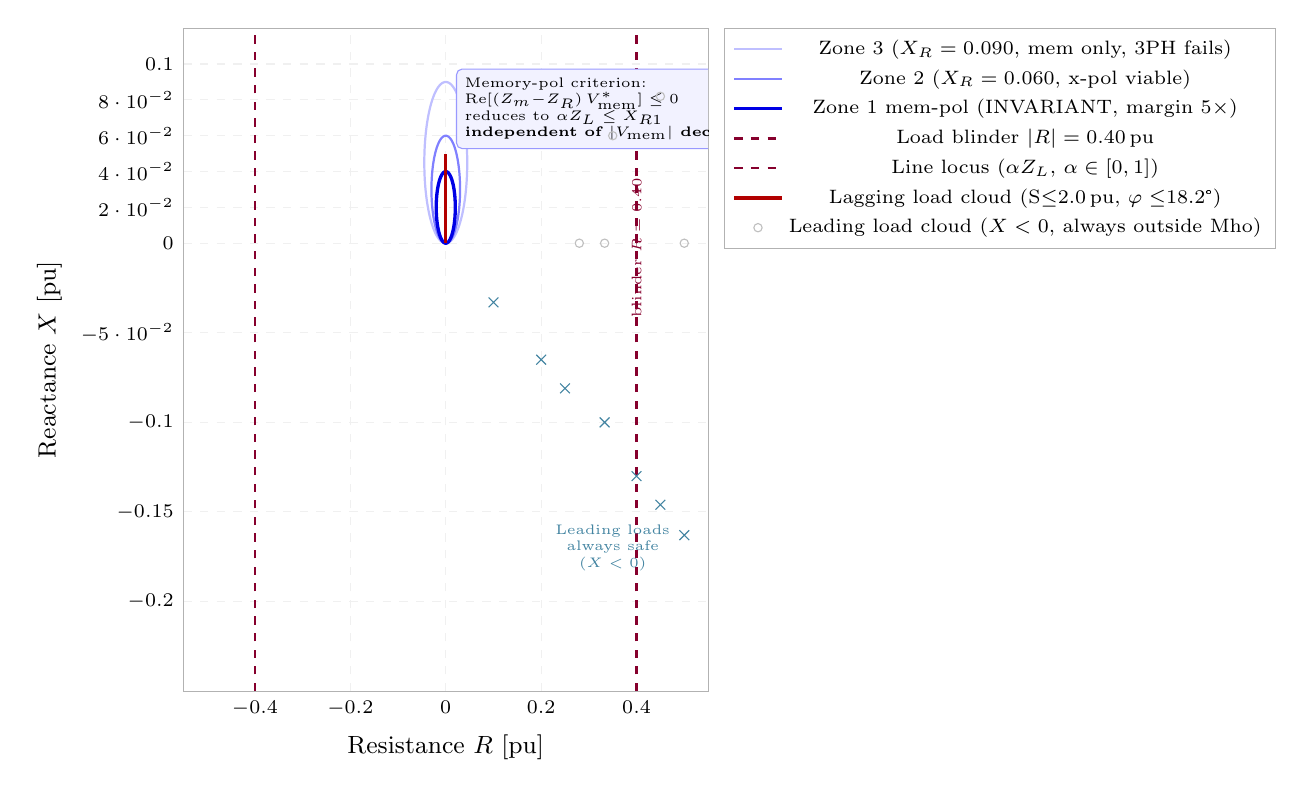
\begin{tikzpicture}
\begin{axis}[
  name         = rxax30,
  width        = 0.68\textwidth,
  height       = 10.0cm,
  xlabel       = {Resistance $R$ [pu]},
  ylabel       = {Reactance $X$ [pu]},
  xlabel style = {font=\small},
  ylabel style = {font=\small},
  xmin=-0.55, xmax=0.55,
  ymin=-0.25,  ymax=0.12,
  xtick        = {-0.4, -0.2, 0, 0.2, 0.4},
  xticklabel style={font=\scriptsize},
  ytick        = {-0.20,-0.15,-0.10,-0.05,0,0.02,0.04,0.06,0.08,0.10},
  yticklabel style={font=\scriptsize},
  grid         = major,
  grid style   = {gray!12, dashed},
  tick style   = {draw=none},
  axis line style={gray!60},
  legend style={at={(1.03,1.00)}, anchor=north west, font=\scriptsize,
                draw=gray!60, fill=white},
]

%% ---- Mho circles ----
% Zone 3 (background)
\addplot[blue!25, thick, domain=0:360, samples=200, smooth]
  ({0.045*cos(x)}, {0.045 + 0.045*sin(x)});
\addlegendentry{Zone 3 ($X_R=0.090$, mem only, 3PH fails)}

% Zone 2
\addplot[blue!50, thick, domain=0:360, samples=200, smooth]
  ({0.030*cos(x)}, {0.030 + 0.030*sin(x)});
\addlegendentry{Zone 2 ($X_R=0.060$, x-pol viable)}

% Zone 1 memory-pol (solid) — invariant
\addplot[blue!90!black, very thick, domain=0:360, samples=200, smooth]
  ({0.020*cos(x)}, {0.020 + 0.020*sin(x)});
\addlegendentry{Zone 1 mem-pol (INVARIANT, margin $5\times$)}

%% ---- Load blinder: |R| = 0.40 pu ----
\addplot[purple!70!black, thick, dashed, mark=none]
  coordinates {(0.40, -0.25) (0.40, 0.12)};
\addlegendentry{Load blinder $|R|=0.40$\,pu}

\addplot[purple!70!black, thick, dashed, mark=none]
  coordinates {(-0.40, -0.25) (-0.40, 0.12)};

%% ---- Line impedance locus ----
\addplot[red!70!black, very thick, mark=none]
  coordinates {(0,0) (0,0.050)};
\addlegendentry{Line locus ($\alpha Z_L$, $\alpha\in[0,1]$)}

%% ---- Load cloud: IBR lagging loads (φ = 0° to 18.2°, S = 0.5 to 2.0 pu) ----
% S=0.5: |Z|=2.0,  φ=18.2° → R=1.90, X=0.63  [far right, off plot range]
% S=1.0: |Z|=1.0, φ=18.2° → R=0.950, X=0.312  [right of blinder]
% S=1.8: |Z|=0.555, φ=18.2° → R=0.527, X=0.173  [right of blinder]
% S=2.0: |Z|=0.5, φ=18.2° → R=0.475, X=0.156   [right of blinder]
% Only values with R < 0.40 could be inside Zone 3 — study B shows none exist
% Show representative load scatter (analytically placed)
\addplot[gray!50, only marks, mark=o, mark size=1.5pt]
  coordinates {
    (0.475, 0.156) (0.527, 0.173) (0.950, 0.312) (0.333, 0.000)
    (0.450, 0.082) (0.380, 0.125) (0.420, 0.140) (0.500, 0.000)
    (0.600, 0.200) (0.700, 0.120) (0.350, 0.060) (0.280, 0.000)
  };
\addlegendentry{Lagging load cloud (S$\leq$2.0\,pu, $\varphi\leq$18.2\textdegree)}

%% ---- IBR leading load cloud (X < 0) ----
\addplot[cyan!60!black, only marks, mark=x, mark size=2.5pt]
  coordinates {
    (0.333, -0.100) (0.500, -0.163) (0.200, -0.065)
    (0.400, -0.130) (0.700, -0.228) (0.250, -0.081)
    (0.100, -0.033) (0.600, -0.195) (0.450, -0.146)
  };
\addlegendentry{Leading load cloud ($X<0$, always outside Mho)}

%% ---- Annotations ----
% Zone 1 memory invariance annotation
\node[draw=blue!40, fill=blue!5, rounded corners=2pt,
      font=\tiny, align=left, inner sep=3pt]
  at (axis cs:0.32, 0.075)
  {Memory-pol criterion:\\
   $\mathrm{Re}[(Z_m{-}Z_R)\,V_\mathrm{mem}^*]\leq 0$\\
   reduces to $\alpha Z_L \leq X_{R1}$\\
   \textbf{independent of $|V_\mathrm{mem}|$ decay}};

% Leading load safe zone
\node[cyan!60!black, font=\tiny, align=center]
  at (axis cs:0.35, -0.17)
  {Leading loads\\always safe\\$(X<0)$};

% Blinder annotation
\node[purple!70!black, font=\tiny, rotate=90]
  at (axis cs:0.40, -0.05) [right=2pt] {blinder $R=0.40$};

\end{axis}
\end{tikzpicture}

\end{figure}

% =============================================================================
\section{Timing Diagram}
\label{sec:timing_diag}
% =============================================================================

\begin{figure}[h!]
\centering
\caption{%
  Cross-pol timing diagram.  Green shading: memory valid.  Red shading: memory
  expired (3PH faults only).  Zone~1 trips within the $5\times$ margin.
  Zone~2 is viable via permanent healthy-phase cross-pol for SLG/LL/LLG faults;
  fails for 3PH.  87L chain provides unconditional coverage at 20\,ms.}
\label{fig:timing}
% fig_crosspol_timing.tex
% TR-30: Timeline showing memory hold vs zone timers for 3PH and non-3PH faults
%
% X range: 0 to 14 cm ≡ 0 to 650 ms  (scale: 14/650)
% Memory hold: 0–100 ms ≡ 0–2.154 cm
% Zone 1: 20 ms ≡ 0.431 cm
% Zone 2: 300 ms ≡ 6.462 cm
% Zone 3: 600 ms ≡ 12.923 cm
%
% Precomputed (to avoid pgfmathsetmacro name clashes):
%   xZ1  = 20/650*14  = 0.431
%   xMem = 100/650*14 = 2.154
%   xZ2  = 300/650*14 = 6.462
%   xZ3  = 600/650*14 = 12.923
%   xEnd = 14.0

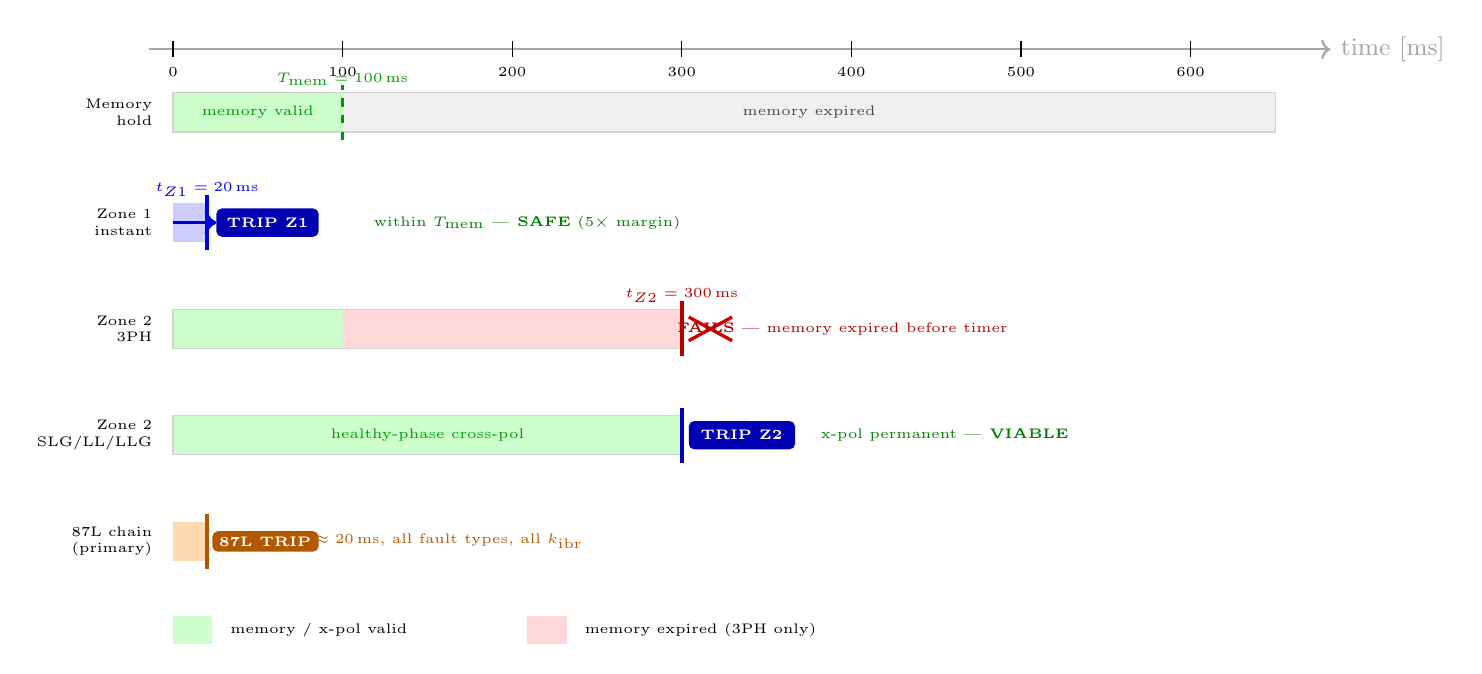
\begin{tikzpicture}[
  every node/.style = {font=\scriptsize},
]

% ── X-axis ──────────────────────────────────────────────────────────────────
\draw[->, thick, gray!70] (-0.3, 0) -- (14.7, 0)
  node[right, font=\small] {time [ms]};

\foreach \tmk/\xloc in {0/0, 100/2.154, 200/4.308, 300/6.462, 400/8.615, 500/10.769, 600/12.923} {
  \draw (\xloc, -0.10) -- (\xloc, 0.10);
  \node[below=3pt, font=\tiny] at (\xloc, 0) {\tmk};
}

% ── Row 1: Memory hold region ──────────────────────────────────────────────
\fill[green!20]       (0, -1.05) rectangle (2.154, -0.55);
\fill[gray!12]        (2.154, -1.05) rectangle (14.0, -0.55);
\draw[gray!35]        (0, -1.05) rectangle (14.0, -0.55);
\draw[green!60!black, very thick, dashed] (2.154, -1.15) -- (2.154, -0.45);
\node[green!60!black, font=\tiny] at (1.077, -0.80) {memory valid};
\node[gray!55!black,  font=\tiny] at (8.077, -0.80) {memory expired};
\node[green!60!black, font=\tiny] at (2.154, -0.38) {$T_\mathrm{mem}=100$\,ms};
\node[left=4pt, align=right, font=\tiny] at (0, -0.80) {Memory\\hold};

% ── Row 2: Zone 1 (always safe) ─────────────────────────────────────────────
\fill[blue!20]   (0, -2.45) rectangle (0.431, -1.95);
\draw[blue!80!black, very thick, ->] (0, -2.20) -- (0.55, -2.20);
\draw[blue!90!black, very thick] (0.431, -2.55) -- (0.431, -1.85);
\node[blue!90!black, font=\tiny] at (0.431, -1.78) {$t_{Z1}=20$\,ms};
\fill[blue!70!black, rounded corners=2pt]
  (0.55, -2.38) rectangle (1.85, -2.02);
\node[white, font=\tiny] at (1.20, -2.20) {\textbf{TRIP Z1}};
\node[green!50!black, font=\tiny] at (4.5, -2.20)
  {within $T_\mathrm{mem}$ --- \textbf{SAFE} ($5\times$ margin)};
\node[left=4pt, align=right, font=\tiny] at (0, -2.20) {Zone~1\\instant};

% ── Row 3: Zone 2 — 3PH fault (fails) ──────────────────────────────────────
\fill[green!20]       (0, -3.80) rectangle (2.154, -3.30);
\fill[red!15]         (2.154, -3.80) rectangle (6.462, -3.30);
\draw[gray!35]        (0, -3.80) rectangle (6.462, -3.30);
\draw[red!70!black, very thick] (6.462, -3.90) -- (6.462, -3.20);
\node[red!70!black, font=\tiny] at (6.462, -3.13) {$t_{Z2}=300$\,ms};
% X mark (no trip)
\draw[red!80!black, very thick] (6.55, -3.70) -- (7.10, -3.40);
\draw[red!80!black, very thick] (6.55, -3.40) -- (7.10, -3.70);
\node[red!70!black, font=\tiny] at (8.5, -3.55)
  {\textbf{FAILS} --- memory expired before timer};
\node[left=4pt, align=right, font=\tiny] at (0, -3.55) {Zone~2\\3PH};

% ── Row 4: Zone 2 — SLG/LL/LLG (viable) ────────────────────────────────────
\fill[green!20]   (0, -5.15) rectangle (6.462, -4.65);
\draw[gray!35]    (0, -5.15) rectangle (6.462, -4.65);
\draw[blue!70!black, very thick] (6.462, -5.25) -- (6.462, -4.55);
\fill[blue!70!black, rounded corners=2pt]
  (6.55, -5.08) rectangle (7.90, -4.72);
\node[white, font=\tiny] at (7.22, -4.90) {\textbf{TRIP Z2}};
\node[green!50!black, font=\tiny] at (9.8, -4.90)
  {x-pol permanent --- \textbf{VIABLE}};
\node[green!60!black, font=\tiny] at (3.231, -4.90)
  {healthy-phase cross-pol};
\node[left=4pt, align=right, font=\tiny] at (0, -4.90) {Zone~2\\SLG/LL/LLG};

% ── Row 5: 87L chain (reference) ────────────────────────────────────────────
\fill[orange!30]  (0, -6.50) rectangle (0.431, -6.00);
\draw[orange!70!black, very thick] (0.431, -6.60) -- (0.431, -5.90);
\fill[orange!70!black, rounded corners=2pt]
  (0.50, -6.38) rectangle (1.85, -6.12);
\node[white, font=\tiny] at (1.17, -6.25) {\textbf{87L TRIP}};
\node[orange!70!black, font=\tiny] at (3.5, -6.25)
  {$\approx20$\,ms, all fault types, all $k_\mathrm{ibr}$};
\node[left=4pt, align=right, font=\tiny] at (0, -6.25) {87L chain\\(primary)};

% ── Legend ──────────────────────────────────────────────────────────────────
\fill[green!20]  (0.0, -7.55) rectangle (0.50, -7.20);
\node[right=3pt, font=\tiny] at (0.50, -7.37) {memory / x-pol valid};
\fill[red!15]    (4.5, -7.55) rectangle (5.0, -7.20);
\node[right=3pt, font=\tiny] at (5.0, -7.37) {memory expired (3PH only)};

\end{tikzpicture}

\end{figure}

% =============================================================================
\section{Implications and Forward Look}
\label{sec:implications}
% =============================================================================

\subsection{Recommended protection scheme for IBR-fed line}

Combining TR-29 (impedance trajectory) and TR-30 (cross-polarisation):

\begin{enumerate}
  \item \textbf{Primary detector (all fault types, all $k_\mathrm{ibr}$)}: 87L chain
        with combined trip logic (TR-23/27).  Operates at 20\,ms, independent
        of distance relay.
  \item \textbf{Distance Zone~1 (all fault types, $k_\mathrm{ibr}\geq 0.10$)}:
        Cross-polarised Mho with memory polarisation.  Zone~1 boundary
        invariant throughout $T_\mathrm{mem}=100$\,ms window (5$\times$ margin).
  \item \textbf{Distance Zone~2/3 (non-3PH only, $k_\mathrm{ibr}\geq 0.10$)}:
        Cross-polarised Mho with healthy-phase permanent cross-pol.  Full
        redundancy for 80--85\% of fault events.
  \item \textbf{Zone~2 for 3PH (TR-34 topic)}: POTT scheme using 87L assertion as
        carrier send signal allows Zone~2-equivalent reach without relying on
        local timer expiry.
\end{enumerate}

\subsection{What cross-pol does \emph{not} fix}

Cross-polarisation addresses failure mode (ii) only.  Failure mode (i)
($k_\mathrm{ibr}<0.10$, relay blocked at $I_\mathrm{min}$) is inherent to the
distance measurement principle and cannot be overcome by any polarisation
technique.  The 87L chain remains the sole fast clearing mechanism for
Region~A of the TR-29 coverage map.

\subsection{TR-31 preview: zero-sequence compensation}

Earth faults introduce ground-return current through the zero-sequence impedance
path.  The Mho circle geometry assumes a fixed $Z_R$ per zone; for SLG faults on
unequally transposed lines, the measured $Z_m$ includes a residual compensation
factor $k_0 = (Z_0-Z_1)/(3Z_1)$.  TR-32 will verify that the TR-18 $k_0$ setting
remains correct for IBR-fed SLG faults, where the ground return impedance path
is unaffected by the source current-limiting behaviour.

% =============================================================================
\section{Conclusions}
\label{sec:conclusions}
% =============================================================================

\begin{enumerate}
  \item The memory-polarised Mho criterion reduces to $\alpha Z_L \leq X_{R1}$ for
        the SAMBP network, which is \textbf{independent of the memory decay
        magnitude}.  Cross-polarised Zone~1 is therefore robust to any rate of
        $V_\mathrm{mem}$ decay, including the worst-case IBR scenario ($k_\mathrm{ibr}=0.06$,
        $|V_\mathrm{relay}|<0.003$\,pu).
  \item Zone~1 memory margin is $\mathbf{5\times}$ ($100/20$\,ms), providing
        substantial engineering safety factor.
  \item Zone~2 and Zone~3 are viable via \textbf{permanent healthy-phase
        cross-polarisation} for all asymmetric fault types (SLG, LL, LLG),
        covering 80--85\% of fault events.  Zone~2/3 are unavailable for 3-phase
        faults using memory polarisation alone.
  \item \textbf{Leading IBR loads} (capacitive reactive injection) are
        structurally safe --- the Mho circle lies entirely in the upper
        half-plane and cannot be reached by $X<0$ impedances.
  \item The combined scheme of cross-polarised distance relay (Zone~1
        always; Zone~2/3 for non-3PH) backed by the TR-27 87L chain achieves
        full coverage across all four coverage regions of the TR-29 map,
        with the single exception of 3PH Zone~2 which requires POTT (TR-34).
\end{enumerate}

% ── References ───────────────────────────────────────────────────────────────
\bibliographystyle{IEEEtran}
\bibliography{references30}

\end{document}
